 
\subsection{Gaia DR2 analysis}

\subsubsection{New vs. old catalog} 


\begin{figure}[t]
\centering
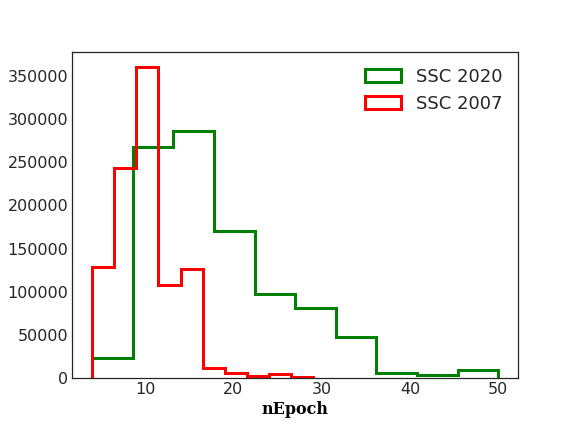
\includegraphics[width=0.4\textwidth, keepaspectratio]{figures/nepoch_compOvsN.png}
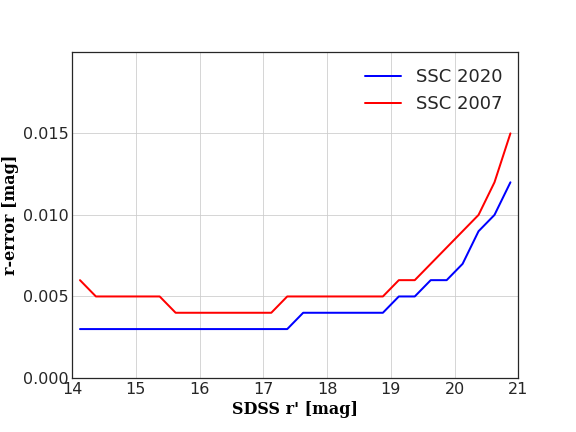
\includegraphics[width=0.4\textwidth, keepaspectratio]{figures/rerr_compOvsN.png}
\caption{{\it Left:} A comparison of the number of observational epochs for matched stars in the 2020 (v3.4) versus 2007 (v2.6) Standard Star Catalog (SSC). {\it Right:} A comparison of the median formal $r$ band photometric uncertainties of matched objects in the 2020 versus 2007 SSC, as a function of their $r$ magnitudes.
\label{fig:rerr_nvso}}
\end{figure}

There are meaningful improvements, but still within the stated accuracy of the original catalog 
claimed in \pO. 

\begin{figure}[t]
\centering
\includegraphics[width=0.8\textwidth, keepaspectratio]{GaiaRApm.png}
\caption{TO BE REDONE. The top panel shows the R.A. difference between SDSS and Gaia 
vs. R.A. proper motion reported by Gaia. The solid line shows the median difference in bins 
of proper motion and the dashed lines mark the $\pm 2 \sigma_G$ envelope around the medians,
where $\sigma_G$ is the robust standard deviation\footnote{We use robust estimator of standard deviation
computed as $\sigma_G = 0.741*(q_{75}-q_{25})$, where $q_{25}$ and $q_{75}$ are the 25\% and 75\% quantiles, 
and the normalization factor 0.741 assures that $\sigma_G$ is equal to standard deviation for normal (Gaussian) 
distribution.}. The botom panel shows the R.A. difference after correcting using the best-fit R.A. difference vs. 
proper motion curve, as a function of SDSS $r$ magnitude. As evident, the residual differences are dominated 
by systematic errors in SDSS astrometry at the level of $\sim30$ milliarcsec (note that there is no increase with 
magnitude). Analogous plots for using Declination quantities are similar. 
\label{fig:GaiaRApm}}
\end{figure}
  

\begin{figure}[t]
\centering
\includegraphics[width=0.8\textwidth, keepaspectratio]{dmResid2b_dr_RA_Dec.png}
\caption{TO BE REDONE. The differences between the $r$ band magnitudes reported in the
first release of the catalog (v2.6) and the version reported here (v3.2). Dots in the left panel
show the data, the thick solid line is the median for bins of R.A. and the two thin solid lines
mark the $\pm 2 \sigma_G$ envelope around the median , where $\sigma_G$ is the robust standard 
deviation. The two dashed lines at $\pm 0.01$ mag are added to guide the eye. The right panel
is analogous, except that the $r$ magnitude differences are binned by Declination. The periodic
pattern shows the imprint of the SDSS photometric calibration telescope and is due to errors in 
applied flat-field corrections. The contribution of these errors to photometric zeropoint variation 
in the first catalog release is about 6 millimag rms (root-mean-square scatter). 
\label{fig:dmResid2b_dr_RA_Dec}}
\end{figure}
   
 
\begin{figure}[t]
\centering
\includegraphics[width=0.8\textwidth, keepaspectratio]{dmResid4_dgi_RA_Dec.png}
\caption{TO BE REDONE.  Analogous to Figure~\ref{fig:dmResid2b_dr_RA_Dec}, except that here 
the differences in the SDSS $g-i$ color are shown instead of the $r$ band magnitude. 
The median differences are by and large confined to the $\pm 0.01$ mag range. 
\label{fig:dmResid4_dgi_RA_Dec}}
\end{figure}
  
  

\subsubsection{Comparison to Gaia Gmag photometry} 


\begin{verbatim}

- show photometric residuals relative to Gaia in RA and Dec directions  

Residuals for Gaia G minus SDSS G (from gri): this one vs. RA shows that one can 
now reproduce Gaia’s G w/o systematics (in Dec residuals are even smaller):
Gresid_RA.png 

Similarly, RA and Dec systematics for the g-i color generated from 
Gaia’s BP-RP are also very small 
colorResid2b_gi_RA.png

Note that I am selecting and showing only a small subset of all plots 
that I looked at! 


- show a problem with Gaia photometry at G~16 and trend at fainter magnitudes

There are weird systematics wrt Gaia’s G mag for both magnitude and
color residuals: 
Gresid_Gmag.png
colorResid2_gi_Gmag.png

I don’t think these are due to SDSS photometry, because...

- show systematic differences between Gaia’s G and (BP, RP) photometry  

even when *only* Gaia data are used (to predict Gmag from BP and RP) there 
are even larger systematics: 
these are HUGE! 
colorResid2_GRP_RA.png
no systematics here because of bin size: 112 deg by 0.05 deg
colorResid2_GRP_Dec.png

but again HUGE systematics at the faint end: 
colorResid2_GRP_Gmag.png

I conclude that Gmag has a bit of a problem at G~16 (a 3 milimag jump, a known
effect in DR1, I thought they’d fix it in DR2) and ~0.01-0.02 at the faint end (G~20). 
BP and RP have a much larger problem at the faint end (a bias of ~0.05 mag). More 
details when I start describing this analysis in the manuscript. The bottom line is 
that the new catalog is demonstrably good and better than the old one! 

\end{verbatim}


\subsubsection{Comparison to Gaia BP and RP photometry} 


The idea is simple: 
\begin{itemize}
\item Fit the SDSS $g-r$, $r-i$ and $r-z$ colors as functions of the Gaia $BP-RP$ color
\item Using these best-fits, synthesize Gaia-based $g-r$, $r-i$ and $r-z$ colors for 
each star
\item Compare and quantify residuals between SDSS and Gaia-based $g-r$, $r-i$ and $r-z$ 
        colors by binning them by RA, Dec and mag and examining for systematics
\end{itemize}

In all three colors the maximum systematics do not exceed 0.01 mag, and the rms
for systematics is $<$7 milimag: 


\begin{deluxetable}{l|c|c}[t]
\tablecaption{The robust standard deviation for binned SDSS-based vs. Gaia-based color residuals$^a$. \label{tab:Gaia2}}
\tablehead{
\colhead{Color } & \colhead{rms for R.A.} & \colhead{rms for Dec}
}
\startdata
  $g-r$     &  3.9      &    4.6   \\
  $r-i$      &  3.3      &    2.9   \\ 
  $i-z$     &   6.7     &    5.3    \\ 
\enddata
\tablenotetext{a}{The robust standard deviation is estimated using interquartile range. The units are millimag.} 
\end{deluxetable}
 

The first two attached plots illustrate this analysis for the g-r color. The yellow dots
in the first plot show the median SDSS g-r color as a function of Gaia’s BP-RP color. 
I simply used linear interpolation of yellow dots to assign Gaia-based g-r colors for
each star. The following two plots show residuals in the RA and Dec directions for
the g-r color. Other two colors look similar, with the rms values listed above.

Gaia’s colors are not good enough to predict the u-r color, but I get surprisingly good 
behavior for the u-r color (rms of 0.02 mag and 0.01 mag for RA and Dec, which 
should be very robust upper limits for systematic errors). 

Now two interesting findings. First, I was surprised to learn that Gaia’s G on the
one hand, and BP and RP magnitudes on the other, are more inconsistent than 
I expected. The reason is that G mags are based on forced point source spread function 
fitting, while BP and RP are based on (rectangular) aperture photometry and thus 
suffer from source blending. The systematic differences can often exceed 0.01 mag 
when binned in RA (that is, in about 1 deg by 2 deg patches), and also show strong 
systematics (0.05 mag) at the faint end (that is, vs. magnitude). 

The third attached plot shows the plot of G-RP residuals (GRPresid, where the model 
G-RP is estimated using BP-RP color) vs. RA and Dec. As you see, the variation is 
much stronger for RA and for Dec. The reason is that bins are about 1 deg by 2 deg 
patches for the former and 110 deg by 0.05 deg for the latter. It must be that Gaia has 
systematics on about degree large angular scales that get averaged for the latter
(Dec) but not for the former (RA). 

The last attached plot shows the plot of G-RP residuals vs. Gmag. You can see very
large (>0.01 mag) systematics for Gmag>19. While discrepancies between Gmag
and BP/RP across the sky have been reported in Gaia DR2 documentation, I have
not seen any reports about this magnitude dependence. 

Note that this plot doesn’t use any SDSS data. However, the variation of residuals
for SDSS colors shows very similar dependence vs. magnitude (not attached) and 
thus I think what we see (at the level of 0.02 mags at the faint end) is due to Gaia 
problems, rather than due to problems in SDSS photometry (both old and new 
catalogs show the same effects, so it’s not a bug in Karun’s code either!). 

The second interesting finding is that Gaia didn’t fix a problem they had at G~16
in DR1. They switch between two different algorithms (I forget why something to 
do with their scanning and SNR) and introduce a shift of about 0.005 mag in Gmag 
magnitudes. We clearly see that effect but we cannot yet estimate its significance 
because something is fishy with our photometric uncertainty estimates in the new 
catalog.  



\subsection{Pan-STARRS analysis}


\subsection{DES analysis}


